\section{1978: 2nd Generation Microprocessors}
In hindsight it is staggering what extra efforts and complications had to be devised
and endured, because the current technology was not quite sufficient. Also the
engineers at Xerox underwent the same fate, but knowingly and willingly. They
knew that in a few years much more powerful technology would be available. If
they succeeded in building an advanced PC (although at high cost) that would be
much cheaper in the foreseeable future, they could develop advanced system
technology and appropriate software at the present time, gaining a distinct
advantage over competitors later on.

This "philosophy" stood behind the computer Dorado, built with ECL technology in
1984/5. Emitter-coupled logic was very fast, but consumed a very large amount of
power, requiring extensive cooling. But circumstances changed, and the famous
Dorado never delivered what the designers had hoped. A consequence was the
departure from the concept of your own, PC on or under the table, pioneered at
PARC. All Dorados had to be stuffed into an air-conditioned room and were
connected with individual cables throughout the building - not a bus like Ethernet
- to the users.

However, while Alto, Dorado, and others were designed at Xerox, the rest of the
world also moved forward. The companies which had pioneered the 8-bit
micro-processors had now moved to 16-bit, and soon even to 32-bit processors on a
single chip. They did not follow the path to faster, higher-current semiconductor
technologies, but rather to the low-power CMOS FET technology. Thus emerged
in 1978 Intel 8086 processor chip (whose successors dominate the market until
today), and also Motorola 68000.
\begin{figure}[h!]
  \centering
  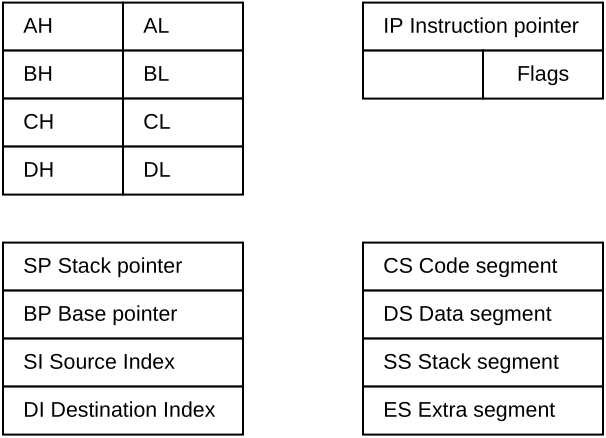
\includegraphics[width=.9\textwidth]{i/5}
  \caption{8086 Register Set}
\end{figure}
 
In particular the Intel part suffered severely under the scarcity of on-chip resources,
resulting in a large variety of special-purpose registers and addressing tricks. The
latter was due to the restriction of 16-bit word and the demand for 20-bit
addresses. This gave rise to the horrid scheme of memory segments and
segmented addressing, a pain for compiler designers and a source of many
inefficiencies. The later 68000 was a much cleaner design, but the Intel part had
already gained the market. The 68000 became the core of the famous Apple
Macintosh, the toy with the small display that looked like a toaster.
